\section{Percabangan (\textit{Banching})}
\newthought{Percabangan} dibutuhkan ketika terdapat beberapa kemungkinan keputusan yang mungkin dalam alur program. Setiap kemungkinan tersebut bergantung terhadap nilai variabel ataupun berdasarkan hasil evaluasi \textbf{kondisi logika}. 

Kondisi logika adalah perbandingan dua atau lebih variabel dengan menggunakan operator logika sebagai berikut.
\begin{enumerate}
	\item Lebih besar ($>$)
	\item Lebih kecil ($<$)
	\item Lebih besar sama dengan ($\geq$)
	\item Lebih kecil sama dengan ($\leq$)
	\item Sama dengan ($==$)
	\item Tidak sama dengan (!= atau $<>$)
\end{enumerate}

Untuk menggabungkan beberapa kondisi logika digunakan \textbf{gerbang logika}\sidenote{Gerbang logika merupakan rangkaian dengan satu atau lebih sinyal masukan yang diproses untuk menghasilkan sinyal keluaran. Contoh gerbang logika adalah AND, NOT, OR, NOR, NAND dan XOR.}.\\
Hasil dari Percabangan dapat berupa dua nilai, Benar (\textit{True}) atau Salah (\textit{False}).

Contoh kondisi logika bisa dilihat di Contoh \ref{cth:kondisiLogika}.
\begin{contoh}
\label{cth:kondisiLogika}
\textbf{Kondisi Logika}\\

\begin{table}\index{typefaces!sizes}
	\centering
	\begin{tabular}{  l  c  }
	\hline
	Kondisi & Hasil \\
	\hline
	7 $>$ 3 & Salah \\
	8 $<$ 8 & Salah \\
	(5 $>$ 9) AND Benar & Salah \\
	(10 $<$ 2) OR (8 $\leq$ 8) & Benar \\
	NOT (3 $<$ 7) & Salah \\
	\hline
	\end{tabular}
\label{table:tabellogika}
\end{table}
\end{contoh}


\subsection{Struktur percabangan}
Percabangan biasanya menggunakan pernyataan \textbf{jika} (\textit{if}). Struktur pernyataan \textit{if} dalam bentuk pseudocode dapat dilihat sebagai berikut.

\begin{tabbing}
~~~~~\=\textbf{if} kondisi 1 \textbf{then}~~~~~~~~~~~~~~~\=\#Pengujian kondisi\\
\>~~~$<$\textbf{statements 1}$>$ \> \#Jika True jalankan\\
\>\textbf{else if } kondisi 2 \textbf{then}\>\#Opsional\\
\>~~~$<$\textbf{statements 2}$>$\>\\
\>\textbf{else}\>\#Opsional\\
\>~~~$<$\textbf{statements 3}$>$\>\\
\>\textbf{end if}
\end{tabbing}

\FloatBarrier
Contoh penggunaan statement \textit{IF} adalah sebagai berikut.

\begin{contoh}
	\textbf{Penggunaan IF..THEN..ELSE}
	\begin{algorithm}[H]
		\caption{PENENTUAN-NILAI()}
		\begin{algorithmic}[1]
		\IF{$x > 4$} 
			\STATE $y = 5$ \COMMENT{Perintah ini hanya dijalankan jika nilai $x > 4$.}
		\ELSIF{$x > 2$}
			\STATE $y = 8$ \COMMENT{Perintah ini hanya dijalankan jika nilai $2 < x < 4$.}
		\ELSE
			\STATE $y = 6$ \COMMENT{Perintah ini hanya dijalankan jika nilai $x \leq 4$.}
		\ENDIF
		\end{algorithmic}
	\end{algorithm}
\end{contoh}


Dalam bentuk flowchart, bisa dilihat di Gambar \ref{fig:flowchart-IF}.

\begin{marginfigure}%
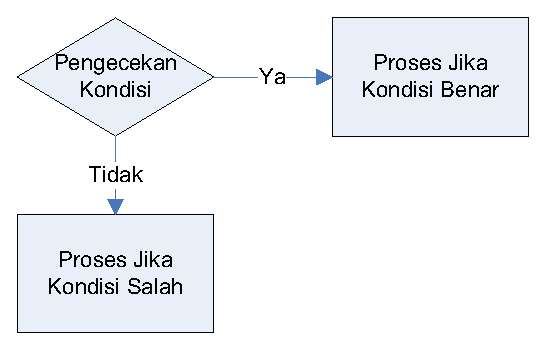
\includegraphics[scale=0.6]{fig/flowchart-IF.eps}%
\caption{Flowchart dari \textit{IF Statement}}%
\label{fig:flowchart-IF}%
\end{marginfigure}

Format \textit{IF Statement} dalam Python bisa ditulis sebagai berikut.

\begin{tabbing}
~~~~~\=\textbf{if} $<$test1$>$:~~~~~~~~~~~~~~~\=\#Pengujian kondisi\\
\>~~~$<$statements1$>$ \> \#Jika True jalankan\\
\>\textbf{elif} $<$test2$>$:\>\#Opsional\\
\>~~~$<$statements2$>$\>\\
\>\textbf{else}:\>\#Opsional\\
\>~~~$<$statements3$>$\>\\
\end{tabbing}

Contoh program Python untuk mengecek bilangan genap atau ganjil bisa dilihat di Listing \ref{lst:genapDanGanjil}.

\begin{listprog}{genapDanGanjil.py}
	\label{lst:genapDanGanjil}
	\begin{lstlisting}[language=Python]
		num = input("Masukkan sebuah angka")
		if num%2 == 0:
				print num, " adalah bilangan genap."
		else:
				print num, " adalah bilangan ganjil."
	\end{lstlisting}
\end{listprog}


\subsection{Percabangan Bersarang (\textit{Nested branching})}
Sebuah percabangan dapat memiliki percabangan di dalamnya dan percabangan yang di dalam tersebut juga dapat memiliki percabangan lainnya di dalam. Sturuktur percabangan bersarang dapat dilihat pada pseudocode berikut.

\begin{tabbing}
~~~~~\=\textbf{if} kondisi 1 \textbf{then}~~~~~~~~~~~~~~~\=\#Pengujian kondisi\\
\>~~~\textbf{if} kondisi 1a \textbf{then}~~~~~~~~~~~~~~~\=\#Pengujian kondisi\\
\>~~~~~~$<$\textbf{statements}$>$ \> \#Jika True jalankan\\
\>~~~\textbf{else}\>\#Opsional\\
\>~~~~~~$<$\textbf{statements}$>$\>\\
\>~~~\textbf{end if}\\
\>\textbf{else if } kondisi 2 \textbf{then}\>\#Opsional\\
\>~~~$<$\textbf{statements 2}$>$\>\\
\>\textbf{else}\>\#Opsional\\
\>~~~$<$\textbf{statements 3}$>$\>\\
\>\textbf{end if}
\end{tabbing}

